% This is samplepaper.tex, a sample chapter demonstrating the
% LLNCS macro package for Springer Computer Science proceedings;
% Version 2.20 of 2017/10/04
%
\documentclass[runningheads]{llncs}
%
\usepackage{graphicx}
\usepackage{tabularx}
% Used for displaying a sample figure. If possible, figure files should
% be included in EPS format.
%
% If you use the hyperref package, please uncomment the following line
% to display URLs in blue roman font according to Springer's eBook style:
% \renewcommand\UrlFont{\color{blue}\rmfamily}

\begin{document}
%
\title{Towards automated provenance collection for experimental runs of agent-based models\thanks{Supported by The Scottish Government}}
%
%\titlerunning{Abbreviated paper title}
% If the paper title is too long for the running head, you can set
% an abbreviated paper title here
%
\author{Doug Salt\inst{1}\orcidID{0000-1111-2222-3333} \and
Gary Polhill\inst{2,3}\orcidID{1111-2222-3333-4444} }
%
\authorrunning{F. Author et al.}
% First names are abbreviated in the running head.
% If there are more than two authors, 'et al.' is used.
%
\institute{The James Hutton Institute, Craigiebuckler Aberdeen AB15 8QH Scotland
\email{doug.salt@hutton.ac.uk}\\
\url{http://hutton.ac.uk}
}
%
\maketitle              % typeset the header of the contribution
%
\begin{abstract}
The abstract should briefly summarize the contents of the paper in
15--250 words.

\keywords{First keyword  \and Second keyword \and Another keyword.}
\end{abstract}
%
%
%
\section{Introduction}

Replication of social simulation results has been highlighted as a significant
issue for the ABM for a number of years (e.g.  \cite{edmonds2003replication}),
and in particular the paper that forms the basis of this work
\cite{polhill2017lessons}.  The focus of replication work has previous just
been on the model itself, but as was shown in ibid, the analysis of the
outputs of the model can potentially be just as complex, and no less difficult
to replicate unless adequate records are kept. Indeed there as an additional
attempt to reproduce the results and even with the lessons learnt from ibid, it
still took months to recreate the final diagrams that were submitted to paper.
The TRACE protocol \cite{schmolke2010ecological,ayllon2021keeping} provides
some guidance highlighting the need to keep a notebook of the analysis done and
a standardised approach to making that notebook; however, the lessons learned
from the replication exercise in \cite{polhill2017lessons} show that more
detailed guidance on the information that should be recorded.  and on tools
that could be used to support the process. Ideally the aim should be to
completely automate the process, record accurately sources of data used,
version check applications used essentially providing a complete graph from
data to result.

The output analysis replication in this paper concerns earlier work with
FEARLUS-SPOMM, which is a coupled agent-based model of agricultural decision-
making and species stochastic patch occupancy metacommunity model that has been
used to explore incentivisation strategies to improve biodiversity (Polhill et
al. 2013; Gimona and Polhill 2011). Belonging to the ‘typification’ class of
social simulations adfa, p. 1, 2011.  © Springer-Verlag Berlin Heidelberg 2011
(“theoretical constructs intended to investigate some properties that apply to
a wide range of empirical phenomena that share some common features” – Boero
and Squaz- zoni, 2005). This work involved the analysis of the outputs from
around 20,000 runs of the model using a number of techniques aimed at
demonstrating nonlinearities in the relationship between incentivisation and
biodiversity outcome.  Recording workflow data on the process used to create
analysis can be challenging, and currently there are no codified standards as
to how this should be done for ABMs. For FEARLUS-SPOMM, the methods used drew
heavily on statistical techniques available as R packages that are as part of
core R functionality. Although R allows transcripts of interactive terminal
sessions to be saved, the work involved great deal of exploration of different
ways of attempting to visualise and analyse the nonlineari- ties in the model
results, not all of which were likely to be reported in the paper. Such logs
are therefore not the best way to record the means by which the outputs were
analysed, and hence the strategy used was to save each analysis or
visualisation in a(n R) script. Since the output from the (Swarm) software that
generated the output data being analysed used a mixture of text formats, some
Perl scripts were also written to process that output into a CSV file for easy
import into R. When the MIRACLE pro- ject (Parker et al. 2015) provided a
context in which the replication of that analysis was necessary, an opportunity
was created to test the viability of the above strategy.

In the rest of this paper, we describe  a tool for automatically recording
metadata, which can be incorporated into the analysis replication process, and
how this  was used to regenerate some of the figures in Polhill et al. (2013)
and we test a tool to support keeping the records needed to per- form
replication more easily, before making some recommendations in concluding
remarks.

\section{Method}


ne of the aims was to leave as much of the code as unchanged as possible (this differs in approach to FAIR-CLI. develop this, both here and in the discussion.

One of the artefacts of the MIRACLE project \cite{} was the Social Simulation REplication Interface or SSREPI. This is the schema shown 
in \ref{fig:schema}. This schema has evolved since it original conception.
The newest version of this document may be found here \cite{}. This is a
database schema derived from the Dublin Core \cite{weibel2000dublin}, the
standard XML datatypes \cite{biron2004xml} and the PROV-O ontologies \cite{missier2013w3c}. The schema is designed with
agnosticisim towards the underlying database technology and as such has
been implmented both in PostgresSQL \cite{stonebraker1991postgres} and Sqlite3 \cite{sqliteorg2023syntax}.

\begin{figure}
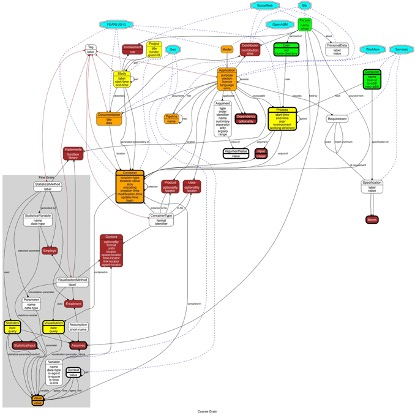
\includegraphics[width=\textwidth]{img/schema.jpeg}
\caption{SSREPI Schema} \label{fig:schema}
\end{figure}


There are two important dimensions of distinction to this schema. First is
fine- versus coarse- grained metadata. Second is provenance versus
workflow. Coarse-grained metadata describes how particular files come (or
came) into being, or were (or could be) used to bring other files into
being. Fine-grained metadata describes specific values recorded in social
simulation outputs. To make the distinction concrete, suppose a simulation
produces a CSV file. The data within the CSV file are covered by
fine-grained metadata, whilst the fact that the simulation produces the
CSV file is coarse-grained. Turning to the other dimension, provenance
metadata describes what actually happens (run W of simulation X produced
output file Y), whilst workflow metadata describes what could happen
(simulation X produces an output file of type Z). The distinctions are
summarised in \ref{fig:finegrain} .

\begin{figure}
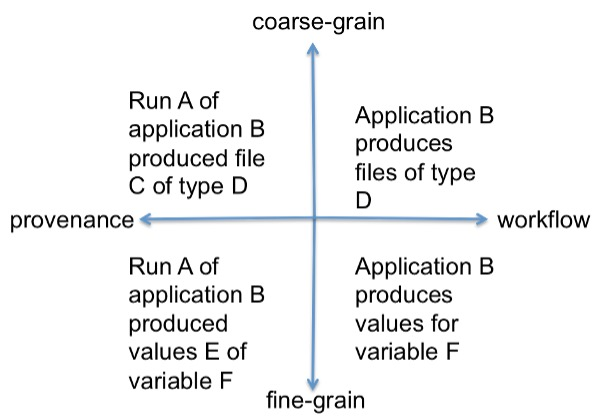
\includegraphics[width=\textwidth]{img/fine-grain-vs-coarse-grain.jpeg}
\caption{Fine grain vs coarse grain provenance} \label{fig:finegrain}
\end{figure}

For the purposes of this short paper we are concentrating on a
demonstration of recording provenance. Indeed we use the example,
mentioned in the introduction of \cite{}, and modified the original Bash \cite{} scripts to include the what we denote as \textit{primitives} . So an example of the code 

In order to record provenance we 
We coded the following primitives from
the SSREPI interface definition \cite{}. These are implemented in a mixture of Python \cite{} and Bash \cite{}

\begin{table}
\caption{Table captions should be placed above the
tables.}\label{tab1}
    \begin{tabularx}{\textwidth}{|l|p{2cm}|p{6cm}|}
\hline
Primitive & Type & Purpose \\
\hline
        SSREPI\_require\_minimum & Metadata & Lower bound on software hardware required \\ SSREPI\_require\_exact & Metadata & Exact bound on software hardware required \\
        SSREPI\_application & Provenance \& Metadata & specifies some executable \\
        SSREPI\_me & Provenance \& Metadata & Determines executable being run or returns a proper reference to the executable being run. \\
        SSREPI\_run & Provenance \& metadata & Blocking invocation of an executable which will allow the specification of all inputs, outputs and arguments. Creates run-time provenance information as well \\
        SSREPI\_batch & Provenance \& metadata & Non blocking invocation of an executable which will allow the specification of all inputs, outputs and arguments. Creates run-time provenance information as well \\
        SSREPI\_argument & Provenance & An argument type to an exectuable \\
        SSREPI\_output & Provenance & An output type from an executable \\
        SSREPI\_input & Provenance & An input type for an exectuable \\
        SSREPI\_hutton\_person & Metadata & Uses our institutions databases to populate metadata for a given individual \\
        SSREPI\_person & Metdata & Provide metadata for a particular actor within this system\\
        SSREPI\_project & Metadata & Specifies a project which contains all studies \\
        SSREPI\_study & Metadata & A set of experiments makes up a single study \\
        SSREPI\_set & Metdata & Sets the default licence and other metadata \\
        SSREPI\_involvement & Metadata & Links personnel to a study \\
        SSREPI\_paper & Metadata & A paper associated with this study \\
        SSREPI\_make\_tag & Metadata & Used for building a folksonomy \\
        SSREPI\_tag & Metadata & Used to tag any entity with a folksonomy tag \\
        SSREPI\_contributor & Metadata & A  person with some kind of relation to an executable or script. \\

        SSREPI\_statistical\_method & Metadata & A statistical method is an approach to computing some statistics. It may be implemented in or as part of an application. A statistical method generates one or more statistical variables as its results, and may use the results of another statistical method in its computation. For example, computing the standard deviation of some data uses the mean of those data. \\
        SSREPI\_visualisation & Metadata & A visualisation is the process of creating an image to depict one or more (typically more than one) values. The results of a visualisation appear in a container.\\
        SSREPI\_statistics & Metadata & Statistics are activities that compute  and populate the values of statistical rvariables. They operate on raw data that are retrieved from the values using a query. To replicate a set of statistics, the query can be rerun, selecting values that are pointed to by containers entries \\
        SSREPI\_visualisation\_method & Metadata & This describes methods for generating visualisations, which then may appear in the content of a container produced by a process running an application that implements it. \\
    
        SSREPI\_implements & Metadata & Links a statistical or visualisation method to an application \\
        SSREPI\_parameter & Metadata & A Parameter is the name of a parameter taken by a statistical or visualisation method, used to configure the way it behaves. \\
        SSREPI\_statistical\_variable & Metadata &  A name for (one of) the result(s) of a statistical method. \\
        SSREPI\_visualisation\_variable & Provenance \& Metadata & Declares a named variable of interest \\
        SSREPI\_variable & Metadata & Names a variable of interest \\
        SSREPI\_statistical\_variable\_value & Provenance \& Metdata & Sets an actual value for a named statistical variable \\
        SSREPI\_value & Provenance & Sets an actual value. This can be connected to any metadata value such         \\ 
        SSREPI\_content & Metadata & Links a kind of output/input/argument to a variable  \\
        SSREPI\_person\_makes\_assumption & Metadata & links a person to an assumption \\
\hline
\end{tabularx}
\end{table}

Broadly speaking SSREPI\_application, SSREPI\_run, SSREPI\_batch, SSREPI\_input,
SSREPI\_output and SSREPI\_argument are responsible for recording coarse grain
provenance. SSREPI\_value, SSREPI\_visualisation\_variable\_value, SSREPI\_statistical\_variable\_value, SSREPI\_run and SSREPI\_batch record fine-grain provenance. The remaining
primitives are largely about recording metadata.

Elaboration of all this may be found in the man pages and design documents in the public repository at git@github.com:DougSalt/ABM-metadata.git

\begin{figure}
\includegraphics[width=\textwidth]{img/workflow.pdf}
\caption{The workflow sub-graph} \label{fig:workflow.pdf}
\end{figure}


\section{Results}

Obviously with complicated diagrams result from the 20,000 runs. The challenge becomes how to visualise these.
There are several graphs produced so far, these being 

We show the workflow graph in fig. \ref{fig:workflow} and a section of the
proveance graph in fig. \ref{fig:sub-provenance}

\begin{figure}
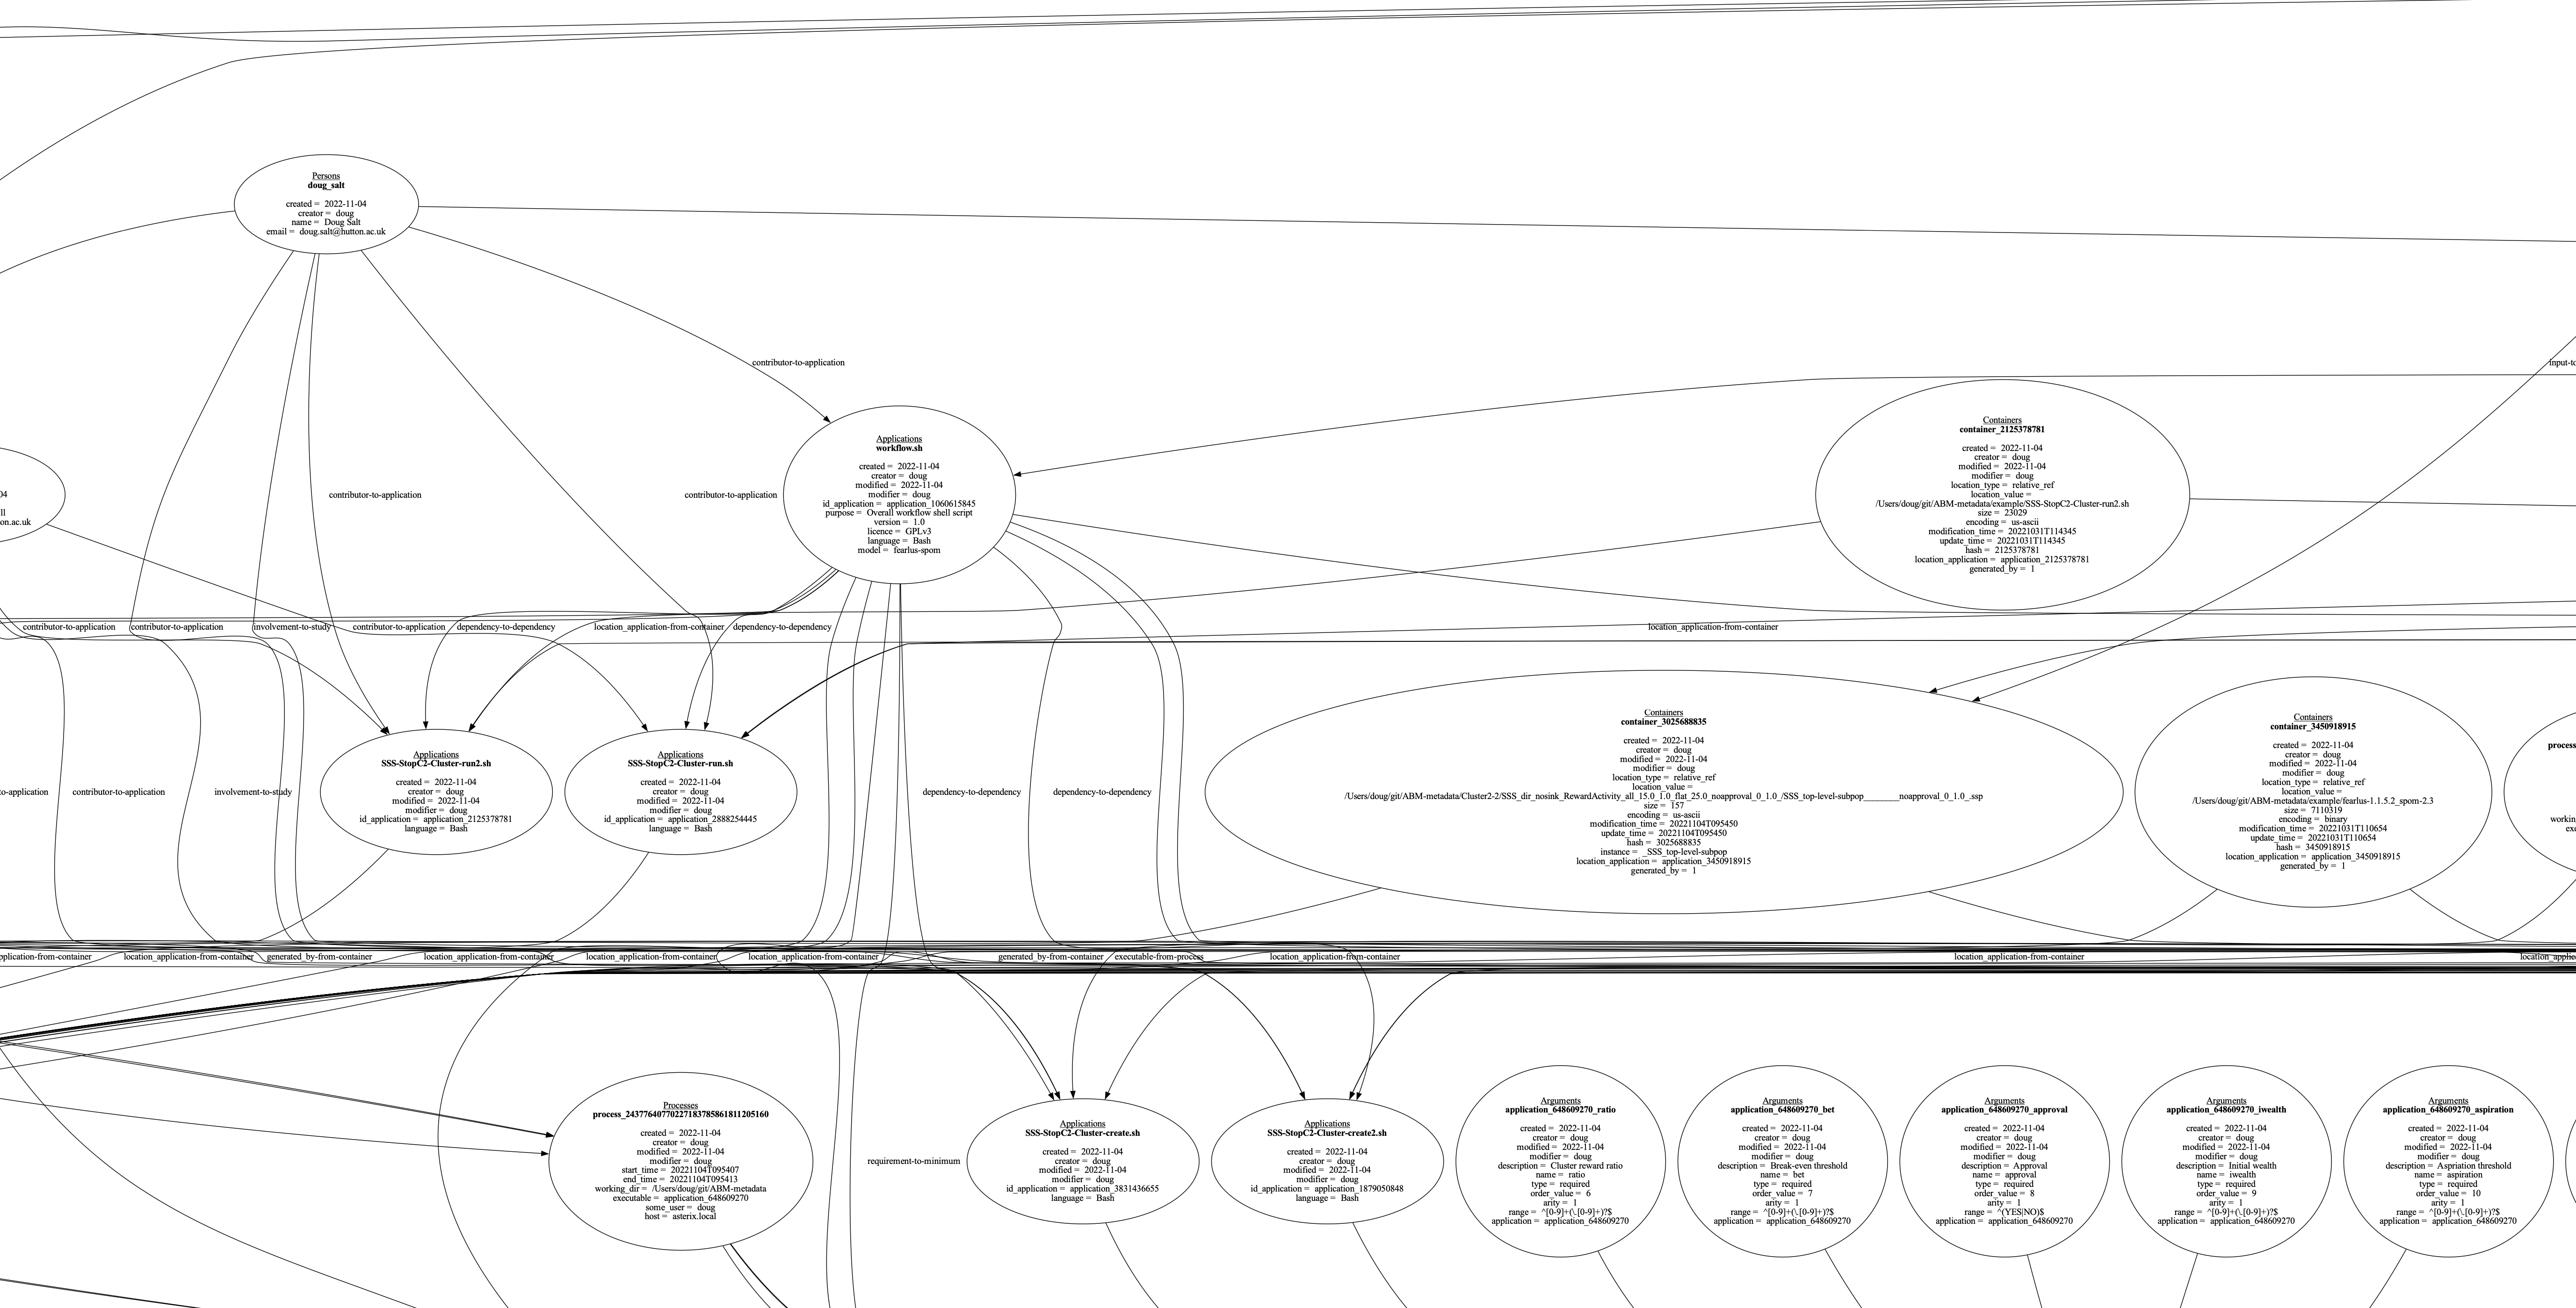
\includegraphics[width=\textwidth]{img/subsection-of-provenance.png}
\caption{A small sub-section of the proevenance graph} \label{fig:sub-provenance}
\end{figure}


\section{Discussion}

What we have learnt from this 
This is a lot of pfaff. and is still not oven ready

So what use is this provenence meta data. Tracing bad data. 

We demonstrate this by tracing a series of bad data across the diagrams.

The proveance should be a directed acyclic graph. There may well be loops in the schema as it stands. The authors have done their best to normalise it to uncover such cycles, but in a schema this complex they may well still exist.


Eventually we should like to take several databases run some machine learning across them to see if there are any commonalities in experiment set up and post processing.

Additionally we want to produce modules in other languages as well, such as R, python and Julia. Especially the latter. 

One of the nice things was that I was able to parallelise the post processing job simply.

%
% ---- Bibliography ----
%
% BibTeX users should specify bibliography style 'splncs04'.
% References will then be sorted and formatted in the correct style.
%
\bibliographystyle{splncs04}
\bibliography[keyword={github.com/DougSalt/MABS2023}]{global.bib}
%
\end{document}
